%%%%%%%%%%%%%%%%%%%%%%%%%%%%%%%%%%%%%%%%%%%%%%%%%%%%%%%%%%%%%%%%%%%%%%%%%%%%%%%%
% Template for USENIX papers.
%
% History:
%
% - TEMPLATE for Usenix papers, specifically to meet requirements of
%   USENIX '05. originally a template for producing IEEE-format
%   articles using LaTeX. written by Matthew Ward, CS Department,
%   Worcester Polytechnic Institute. adapted by David Beazley for his
%   excellent SWIG paper in Proceedings, Tcl 96. turned into a
%   smartass generic template by De Clarke, with thanks to both the
%   above pioneers. Use at your own risk. Complaints to /dev/null.
%   Make it two column with no page numbering, default is 10 point.
%
% - Munged by Fred Douglis <douglis@research.att.com> 10/97 to
%   separate the .sty file from the LaTeX source template, so that
%   people can more easily include the .sty file into an existing
%   document. Also changed to more closely follow the style guidelines
%   as represented by the Word sample file.
%
% - Note that since 2010, USENIX does not require endnotes. If you
%   want foot of page notes, don't include the endnotes package in the
%   usepackage command, below.
% - This version uses the latex2e styles, not the very ancient 2.09
%   stuff.
%
% - Updated July 2018: Text block size changed from 6.5" to 7"
%
% - Updated Dec 2018 for ATC'19:
%
%   * Revised text to pass HotCRP's auto-formatting check, with
%     hotcrp.settings.submission_form.body_font_size=10pt, and
%     hotcrp.settings.submission_form.line_height=12pt
%
%   * Switched from \endnote-s to \footnote-s to match Usenix's policy.
%
%   * \section* => \begin{abstract} ... \end{abstract}
%
%   * Make template self-contained in terms of bibtex entires, to allow
%     this file to be compiled. (And changing refs style to 'plain'.)
%
%   * Make template self-contained in terms of figures, to
%     allow this file to be compiled. 
%
%   * Added packages for hyperref, embedding fonts, and improving
%     appearance.
%   
%   * Removed outdated text.
%
%%%%%%%%%%%%%%%%%%%%%%%%%%%%%%%%%%%%%%%%%%%%%%%%%%%%%%%%%%%%%%%%%%%%%%%%%%%%%%%%

\documentclass[letterpaper,twocolumn,10pt]{article}

% to be able to draw some self-contained figs
\usepackage{tikz}
\usepackage{amsmath}

% inlined bib file
\usepackage{filecontents}

%-------------------------------------------------------------------------------
\begin{filecontents}{\jobname.bib}
%-------------------------------------------------------------------------------

@Book{alireza23,
  author =       {Masrurkhah, Alireza Abed, Amir Seyed Danesh and Seyyedeh Narjes Ghiami Taklimi C.},
  title =        {A survey on implementation of a Linux-based operating system using LFS method},
  publisher =    {International Journal of Computer Science Issues, (IJCSI)},
  year =         2012,
  edition =      {9.00}
}
@Book{arpachiDusseau18:osbook,
  author =       {Arpaci-Dusseau, Remzi H. and Arpaci-Dusseau Andrea C.},
  title =        {Operating Systems: Three Easy Pieces},
  publisher =    {Arpaci-Dusseau Books, LLC},
  year =         2015,
  edition =      {1.00},
  note =         {\url{http://pages.cs.wisc.edu/~remzi/OSTEP/}}
}

@Book{jonathanCorbet19:osbook,
  author =       {Jonathan Corbet and Amanda McPherson},
  title =        {Linux Kernel Development},
  publisher =    {The Linux Foundation},
  year =         2010,
  note =         {\url{http://www.linuxfoundation.org}}
}
@InProceedings{sukumar21,
  author =       {Sukumar B. B, Neelima P. N, and Sunil. Kumar.B},
  title =        {Efficient Round Robin CPU Scheduling Algorithm},
  volume = 4,
  issue = 9,
  year =         2012,
  pages =        {36--42}
  }
@InProceedings{hwang20,
  author =       {Hwang, Lain-Chyr, Steen J. Hsu, San-Yuan Wang, and Yong-Hua Huang},
  title =        {A hybrid scheduling algorithm with low complexity: Jumping Virtual Clock Round Robin},
  booktitle =    {In Distributed Computing Systems Workshops},  
  publisher =    {25th IEEE International Conference (IEEE)},
  year =         2005,
  edition =      {1.00},
  pages =        {698-703},
}
  
\end{filecontents}

%-------------------------------------------------------------------------------
\begin{document}
%-------------------------------------------------------------------------------

%don't want date printed
\date{}

% make title bold and 14 pt font (Latex default is non-bold, 16 pt)
\title{\Large \bf JVCRR Based Scheduler in Linux\\}

%for single author (just remove % characters)
\author{
{\rm Your N.\ Here}\\
Your Institution
\and
{\rm Second Name}\\
Second Institution
% copy the following lines to add more authors
% \and
% {\rm Name}\\
%Name Institution
} % end author

\maketitle

%-------------------------------------------------------------------------------
\begin{abstract}
%-------------------------------------------------------------------------------
Many people have been interested in open-source software and free operating systems. People have neglected to recognise that while installing standard distributions, users are frequently compelled to install a large number of apps that are unlikely to be utilised. These initiatives are a waste of money. The Linux system defines its standard scheduling algorithms, of which the WFC is mostly used. While the defined algorithms go a long way towards optimality, there is still room for improvement, it is impossible to avoid the inclusion of components that will never be used. We can leverage on Linux Kernel Modules and build our custom scheduler, which we can load into the system. We propose a scheduling method called the Jumping Virtual Clock Round Robin, which works as a combination of Dynamic Jumping Virtual Clock and the Static Round Robin Algorithm to provide a much more optimal scheduler to the Linux system.

\end{abstract}


%-------------------------------------------------------------------------------
\section{Introduction}
%-------------------------------------------------------------------------------

The Linux kernel and a collection of software make up a Linux-based distribution. Because the Linux kernel is modular, it includes a scheduler module. The scheduling algorithm is used to create the scheduler module. Fair Scheduling is the scheduling method used in Linux kernel version 2.6. Fair scheduling does not ensure that all jobs will be completed at an O(1) rate. We therefore propose a hybrid algorithm that leverages in the combined effect of virtual clocks, the round Robin Queue and the Jumping Queue.~\cite{alireza23} 

We will build our algorithm as a kernel module, which we will load into the Linux system as an extension, and then run some processes, and evaluate our findings.

We will be following the guidelines specified in the LFS Open Source Tool, LFS is a project that provides all developer guidelines so that they may create their own customised distribution. Linux's modular design makes it the most adaptable operating system and one that can be moved from a small personal computer to a supercomputer. LFS is primarily concerned with the compilation of numerous Linux packages accessible in repositories located all over the globe and brought together over the internet.

Any operating system's efficiency is mostly determined by how quickly it completes tasks. In an operating system, the scheduler module assigns tasks to the kernel based on priority or the shortest job. The scheduling algorithm employed by an operating system determines which job to run next. There are a variety of scheduling algorithms to select from, so picking the right one is vital.

We have a collection of simple algorithms such as the First-Come-First-Served, Shortest Job First, Shortest Job Remaining, and the Higher Response Ration Next algorithm all a combination of pre-emptive and non-pre-emptive algorithms to the more complex ones such as the Weighted Fair Queuing, Virtual Clock, Round Robin, and Jumping Virtual Clock, while we consider them to be inefficient. As each of them need a certain amount of time to carry out any given command. All of the preceding methods have a complexity of around O(log N), which makes them ineffective. Any OS that claims to be more efficient and superior should have at least O (1) complexity.

We are guaranteed a complexity of O(1) if we use scheduling techniques like the Virtual Clock or the Leaf Forward Virtual Clock, they however would cost us a picknextinqueue task of complexity O(log N) and O(log log N), which still lags greatly in modern computing.

Fair scheduling is employed in the current Linux kernel, which is efficient but does not ensure that programmes will be executed at O. (1). As a result, a new scheduling method known as JVCRR, which ensures an O(1) rate, is utilised to boost the overall efficiency of the Linux system.

JVCRR is a hybrid method that combines the Jumping Virtual Clock and Round Robin scheduling algorithms. Calculating virtual time and picking the next queue are both part of this process. Because both computing virtual time and picking the next queue take O(1) time, the overall complexity is O(1) (1). As a result, JVCRR outperforms the other specified scheduling techniques.
%-------------------------------------------------------------------------------
\subsection{Plan}
%-------------------------------------------------------------------------------
We are proposing a project based on extending the linux kernel functionality, and will contain packages that are required for the operating system's fundamental and basic functioning. As a result, excluding the remaining packages reduces the size of the Linux distribution. The proposed system will contain a kernel module that acts as a scheduler and uses the JVCRR scheduling algorithm, which has an O(1) time complexity and provides a much more efficient scheduling than the initial one present in the operating system. Because both of these elements are involved, Linux distributions are much quicker at performing system or user-generated activities.

 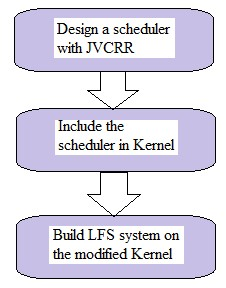
\includegraphics{Article-img/Article-img001.jpg} 

The figure above depicts the overall system flow, or the main processes to take while updating the Linux kernel with JVCRR scheduling. The first step is to create a scheduler by changing the present Linux system's scheduling mechanism. The next stage is to integrate the changed scheduler into the Linux system, which entails replacing the old scheduler with the new one. The LFS system will be built on top of the modified Kernel in the third and final stage.

Because Linux is open source, anybody may readily edit the code, the suggested work was created utilising that distribution. It is also a cost-effective operating system because it is freely accessible. Anyone with access to the internet may readily obtain the source code and make changes. In comparison to other operating systems like as Windows, Linux is more viable in a variety of ways, which is why it is included.

%-------------------------------------------------------------------------------
\section{Description}
%-------------------------------------------------------------------------------
%-------------------------------------------------------------------------------
\subsection{Jumping Virtual Clock}
%-------------------------------------------------------------------------------
Self-Clocked To lower the computational complexity of Virtual Time, Scheduling Helper Algorithms such as Fair Queueing, Virtual Clocks, and Leap Forward Virtual Clock were developed. The utilisation of virtualized Generalized Processor Sharing is not required for Self-Clocked Fair Queueing (GPS). The virtual start time (VST), also known as the virtual finish time (VFT), is set to the virtual end time (VFT) of previously transmitted packets, simplifying the process of calculating the virtual time (VT). This technique, however, has the problem of distributing packets among several queues on the same VST.

Aligning VT in real-time (using a technique like VC) is another way to achieve time complexity O. However because VC can result in an infinite number of rogues, LFVC devised a solution that utilises two lists to track queues that meet and do not satisfy the throughput criterion, respectively, and there are no queues that fulfil the corresponding condition. If VT advances. While VT calculation in LFVC is as complex as in O (1), the two-list structure and condition fulfilment test complicate implementation. According to the literature, the endless fraud and complexity inherent in VT calculations may be overcome by simply designing a real-time VT method based on VT hopping. 

Thus, the rate of VT is often the same as that of actual time, but under specific circumstances, the VT leaps. JVC's goal is to keep things simple while eliminating SCFQ, VC, and LFVC difficulties. JVC's key idea is that, like VC, VT operates in real-time and seizes unique opportunities. JVC's objective is to determine which situation causes the VT to jump. VC rogues can be caused by queue penalties that use more unused bandwidth than allotted, depending on the reason of the rogue. By contrast, a queue that remains idle for a lengthy period of time accumulates and uses them during the subsequent burst. As a result, queues requiring greater bandwidth will be unavailable for brief or extended periods of time, creating an unfair scenario. 

Avoid accumulating credit in the short term for the sake of justice. Thus, each queue evenly divides the bandwidth available at each interval. As a result, if the idle queue becomes clogged, the VT must increment the value to avoid credit build-up. However, these inactive lines will eventually lose what they should have, thus some compensation is necessary. For the reasons stated above and for ease of implementation, when the system status changes, the jump epoch is set to the packet departure time. The system state is defined as the sum of the idle and busy states of all queues. As a result, the JVC's VT rate is similar to that of real-time, except that the VT jumps to the departing packet's VFT upon packet departure if the system's state changes. Following the departure period, fresh busy queue packets may include the brand new and bigger VT, thereby halting credit score accumulation. 

On the other hand, fresh busy queue packets that arrive while the departure packet is being served have a shorter Virtual Time. It is a form of compensation. Because the number of packets that can fit inside a packet's carrier length is often limited, the bias created by employing those packets is also limited. As a result, we will conclude that JVC no longer possesses the exclusive method for computing VT, but also makes other adjustments while keeping the true characteristic. JVC's VT strategy is as follows:

 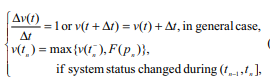
\includegraphics[width=2.7346in,height=0.8543in]{Article-img/Article-img002.png} 

Where v(t) is the VT at time t, tn is the n-th packet of system pn{}'s departure time, and F(pn) is the pn's VFT. VFT is denoted by

 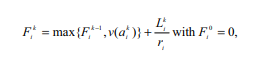
\includegraphics[width=2.7083in,height=0.5937in]{Article-img/Article-img003.png} 

where Fik is the VFT of queue i's k-th packet, pik, with packet length Lik, aik is pik s (actual) arrival time, and ri is queue i's allocation rate. In the first equation, the max function is used to maintain the time approach forward, i.e. the VT will not drop after leaping. When the system's state changes between two departures, i.e. when certain queues switch from idle to busy handling the outgoing packet, the hopping situation arises. The VT notion serves as the foundation for scheduling algorithms that employ VT to determine service order. Additionally, it has an influence on the degree of implementation difficulty. Calculating VT in JVC has a complexity of O(1), which is similar as SCFQ, VC, and LPVC.

On the other side, JVC lacked any disadvantages. Packets arriving in multiple queues during the service time of outbound packets all have the same VT or VFT, as the VT is identical to the outbound packet's VFT prior to the SCFQ. Because the VT approaches in real time in JVC, it will be different if the packet arrives at a different moment, and the likelihood of creating the same VFT will be greatly decreased. JVC also inhibits perpetual fraud due to the fact that VT hopping precludes credit buildup endlessly. Additionally, JVC was relieved of the responsibility of determining the throughput constraint compliance test, the data structure for tracking which queues are high and which are low, or the new VT as an LPVC. Additionally, JVC is simple to use. Because VTs operate in close proximity to actual time, only one system clock is necessary. The same real-time system clock is used to trigger the arrival of VT. If a hop happens, all that is required is to set the VT to the outgoing packet's VFT value.
%-------------------------------------------------------------------------------
\subsection{Jumping Virtual Clock Round Robin }
%-------------------------------------------------------------------------------
With the aid of JVC, Virtual Round Robin Jump Clock reduces the complexity of VT calculation to the lowest achievable O level. If the next queue selection can also be reduced to O, this is the simplest scheduling strategy. As a result, JVC and RR are joined to become JVCRR. While the sequence of services is fixed in RR, the number of services per query may be dynamically modified depending on the input and output criteria. As a result, JVCRR includes a dynamic element known as a service quota that serves as a link between the dynamic VT and the static RR. Quotas are used to track and record the maximum quantity of service that may be delivered to a queue. It is connected to VT since VT is fundamentally a mapping of the number of services available in the queue. When a queue is decommissioned, the quota is adjusted appropriately.
 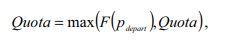
\includegraphics[width=2.4583in,height=0.4689in]{Article-img/Article-img004.png} 
where pdepart is the queue's latest departure packet. Weight Round Robin's quota is comparable to quota (WRR). On the other hand, the weight is defined a priori and statically, but the quota is updated dynamically in response to the queue service situation.
 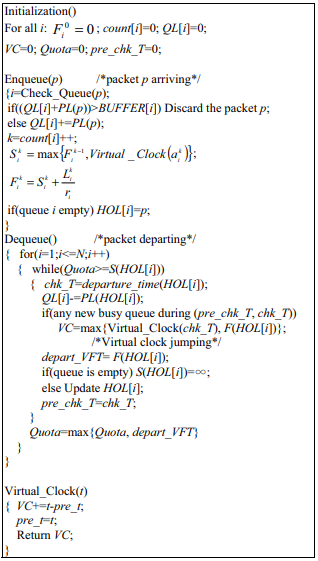
\includegraphics[width=3.3126in,height=5.8437in]{Article-img/Article-img005.png} 
The JVCRR method is illustrated in Figure 1. The Initialization () module is used to initialise system variables. Enqueue () and Dequeue () are two distinct operations that are used to handle incoming and outgoing packets, respectively. VT is calculated in time t by the virtual clock (t) module in a typical scenario. The variables count I QL I VC, chk T, and pre chk T denote the number of packets arriving at queue I, the checkpoint time (that is, the packet's departure time), and pre chk T, respectively. Packet de d\'epart. When packet p arrives, enqueue (p) is invoked. Check Queue (p) finds the index of the queue into which the packet is queued, and then PL (p) assesses if the packet can be queued by increasing the capacity BUFFER I and the length QL I Packet p will be refused if it cannot be queued. When a packet is queued, the length of the queue and the number of arrivals are raised, and the VST kSi and VFT kFi values are computed. Simultaneously, the packet output operation Dequeue () is run. Queues are served sequentially. While the packet is being provided, the jump condition is checked to verify if the VC has been updated. Where F (HOL I denotes a function that denotes the VFT obtained from HOL I After that, HOL I is updated and the quota is reviewed to determine whether there is sufficient room to accommodate another package. For Quota S (HOL I HOL I VST, HOL I (virtual)] has a slower arrival time than the system VT mapped to Quota. As you can see, the HOL I packet has not yet arrived from a VT standpoint, implying that the next queue is responsible.Quotas are adjusted according to Equation 3 before the next queue is served. JVCRR is easy to build due to its simple algorithm. JVCRR is simple, but superior to WFQ, WF2 Q, LFVC, and WRR in terms of performance (next section). The relationship between VST and quotas determines whether the queue will continue to operate. The ability to deliver the package also depends on whether it arrived at this point. Note that JVCRR services are determined by VST, while LFVC, SCFQ, and WFQ services are determined by VFT. VST, on the other hand, is not used to determine the order of services because the order of services has already been determined, but it does determine the amount of services in each query.

%-------------------------------------------------------------------------------
\section{Design }
%-------------------------------------------------------------------------------
\begin{itemize}
\item The user process's process id is first written to the file /proc/process sched add, which corresponds to the kernel module process set. This operation completes a process's registration with the JVCRR Scheduler.
\item The kernel module process scheduler is used to run the JVCRR-based scheduler. For each time quanta, the module does a work queue construct.
\item The kernel module process queue connects the process set and process scheduler modules. The internal details of all the processes connected with the LKM Scheduler are handled by the process queue module. It saves the process information in the form of simple link list nodes.
\item To conduct add, delete, get first, and print actions on the queue, the process queue defines a number of interfaces. Every time quanta, the scheduler executes an add and removal based on the context switch action being triggered.
\item The scheduler pushes the currently executing PID to the process queue via the add to process interface on every time quanta. And, using task-based interfaces, modify its execution from Running to Wait. The process at the front of the queue is picked when the presently running process has been successfully added to the queue. The status of the chosen process is changed to running, and the process is also removed from the queue.
\end{itemize}

%-------------------------------------------------------------------------------
\subsection{Components}
%-------------------------------------------------------------------------------
\begin{itemize}
\item Ubuntu OS
\item make
\item gcc
\end{itemize}

%-------------------------------------------------------------------------------
\subsection{Files included:}
%-------------------------------------------------------------------------------
\begin{itemize}
\item process set.c - source code for configuring a custom scheduler for a process.
\item process scheduler.c - the custom scheduler's source code
\item process queue.c - source code for maintaining the process queue.
\item test pr.c - procedure for executing a custom scheduler.
\item Makefile - This file is used to compile various source code for the LKM scheduler.
\end{itemize}

%-------------------------------------------------------------------------------
\section*{Performance}
%-------------------------------------------------------------------------------

We ran our algorithm under different quantums of 5, 10, 15 and 20, adding a process to the queue every second, and we can see that the execution time increased on an average as the quantum time increased, average time for Quantum(5) was less than all others, with Quantum(10) having the largest average execution time.
 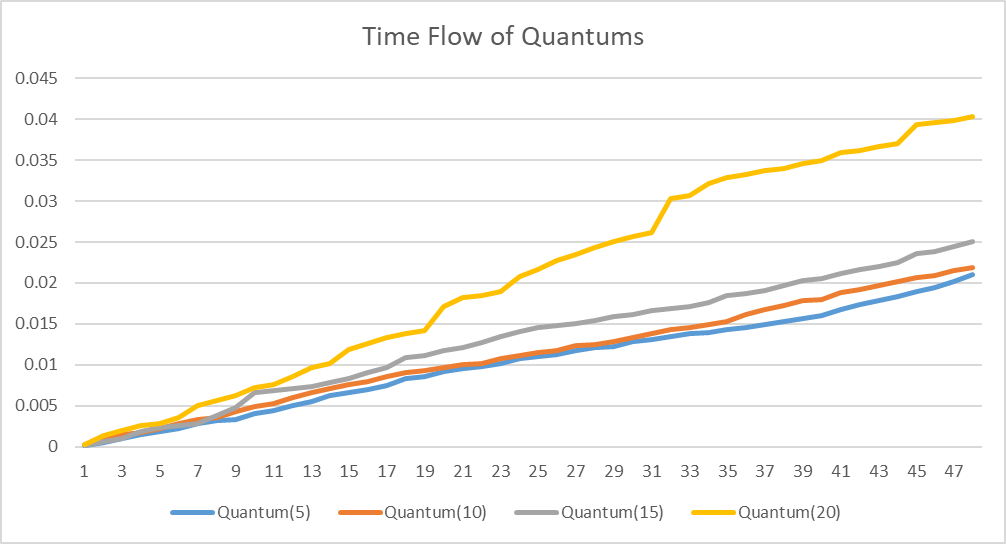
\includegraphics[width=3.4in,height=2.2in]{Article-img/Article-img006.png} 
%-------------------------------------------------------------------------------
\section{References}

Jonathan Corbet, Amanda McPherson, `Linux Kernel Development', The Linux Foundation, \ http://www.linuxfoundation.org, \ Dec 2010. 

Masrurkhah, Alireza Abed, , , and Seyyedeh Narjes Ghiami Taklimi,
 `A survey on implementation of a Linux-based operating system using LFS method' International Journal of Computer Science Issues (IJCSI) 9, no. 2 (2012). 

Hwang, Lain-Chyr, Steen J. Hsu, San-Yuan Wang, and Yong-Hua Huang. `A hybrid scheduling algorithm with low complexity: Jumping Virtual Clock Round Robin',
 In Distributed Computing Systems Workshops, 25th IEEE International Conference on, pp. 698-703. IEEE, 2005. 

Sukumar B. B, Neelima P. N, and Sunil. Kumar.B, `Efficient Round Robin CPU Scheduling Algorithm', volume 4, Issue 9, pp. 36-42, November 2012. 

Robert Love `Linux Kernel Development', Third Edition, ISBN-13: 978-0-672-32946-3, June 2010. 

Gerard Beekmans, `Linux From Scratch', Version 7.4, 2013. \ 

Silberschatz, 2.P. Galvin, and 3.G. O. Gagne, Operating System Concepts, 7th Edition, John Wiley and Sons. INC, 2005.
\end{document}


%%%%%%%%%%%%%%%%%%%%%%%%%%%%%%%%%%%%%%%%%%%%%%%%%%%%%%%%%%%%%%%%%%%%%%%%%%%%%%%%
\end{document}
%%%%%%%%%%%%%%%%%%%%%%%%%%%%%%%%%%%%%%%%%%%%%%%%%%%%%%%%%%%%%%%%%%%%%%%%%%%%%%%%

%%  LocalWords:  endnotes includegraphics fread ptr nobj noindent
%%  LocalWords:  pdflatex acks